\section{Durchführung}
Zu Beginn soll die Zeitabhängigkeit der Schwingungsamplitude untersucht werden, dafür
wird der kleinere der beiden in der Schaltung "verfügbaren" Widerstände verwendet.
Eine Darstellung der verwendeten Schaltung ist in Abbildung \ref{fig:a} zu sehen.
\begin{figure}[H]
  \centering
  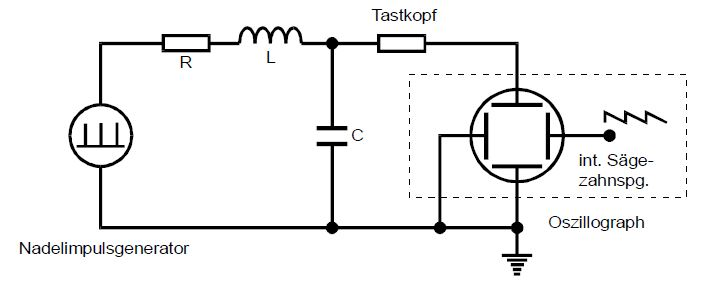
\includegraphics[width=13cm]{a.JPG}
  \caption{Schaltung zur Untersuchung der Zeitabhängigkeit der Ampitude}
  \cite{skript}.
  \label{fig:a}
\end{figure}
Der Schwingkreis wird mit einem Nadelimpuls angeregt. Es ist darauf zu achten, dass
eine erneute Anregung erst erfolgt, wenn die Amplitude der gedämpften
Schwingung um den Faktor 3 bis 8 abgeklungen ist. Auf dem Oszilloskop lässt
sich nun der Verlauf der Schwingungskurve verfolgen und es wird ein
Thermodruck angefertigt.
Der Eingangswiderstand des Oszilloskops kann hier vernachlässigt werden, da der
Tastknopf einen sehr hohen Innenwiderstand ($R_{i}=\SI{10}{\mega\ohm}$) besitzt.

Im Folgenden soll der Widerstand $R_{\text{ap}}$ bestimmt werden, ab dem der apperiodische
Grenzfall eintritt. Dazu wird die Schaltung aus Abbildung \ref{fig:b} verwendet.
\begin{figure}[H]
  \centering
  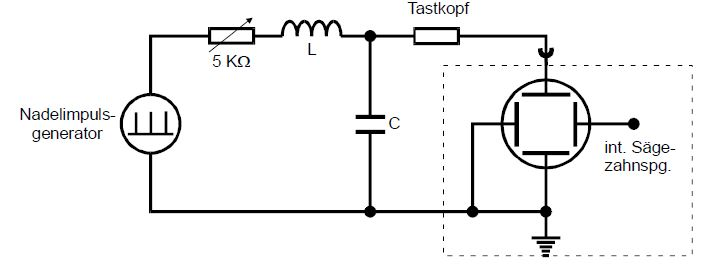
\includegraphics[width=13cm]{b.JPG}
  \caption{Schaltung zur Bestimmung des aperiodischen Grenzwiderstandes $R_{\text{ap}}$}
  \cite{skript}.
  \label{fig:b}
\end{figure}
An dem regelbaren Widerstand wird zunächst ein Maximaler Widerstand eingestellt, sodass
die Kondensatorspannung monoton abnimmt. Nun wird $R$ langsam verringert, bis
am Oszilloskop ein "Überschwingen" zu erkennen ist. Ist dies der Fall, dann wurde
$R_{\text{ap}}$ bereits unterschritten, deshalb wird $R$ wirder vergrößert, bis der
"Überschwinger" verschwindet.

Anschließend wird die Frequenzabhängigkeit der Kondensatorspannung an einem
Serienresonanzkreis untersucht. Dazu wird eine Schaltung wie in Abbildung
\ref{fig:c} zu sehen aufgebaut, außerdem wird der größere der zur Verfügung
stehenden Widerstände verwendet.
\begin{figure}[H]
  \centering
  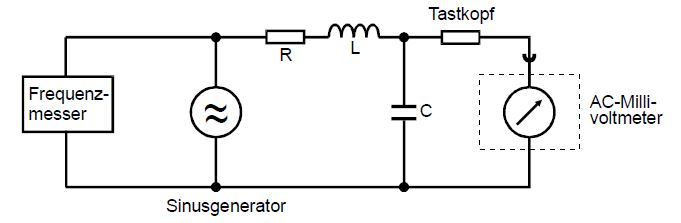
\includegraphics[width=13cm]{c.JPG}
  \caption{Schaltung zurMessung der frequenzabhängigkeit der Kondensatorspannung}
  \cite{skript}.
  \label{fig:c}
\end{figure}
Zunächst wird die Erregerspannung $U$ in abhängigkeit der Frequenz gemessen, diese
ist frequenzabhängig, da sie über den Tastknopf gemessen wird und dessen
Ausgansspannung nicht frequenzunabhängig ist, wie es im Idealfall sein sollte.
Anschließend wird die Kondensatorspannung in Abhängigkeit der Frequenz im Bereich
von 100\;- $\SI{100000}{\Hz}$ gemessen. Im Bereich der Resonanzfrequez werden
dabei mehr Messwerte aufgenommen da dieser Bereich später genauer untersucht werden soll.

Zuletzt wird die Phasenverschiebung $\Phi$ der Kondensatorspannung und
der Erregerspannung gemessen, dazu wird wieder die Schaltung aus Abbildung \ref{fig:c}
verwendet. Wenn beide Spannungsverläufeübereinander angezeigt werden ergibt sich ein Bild
wie in Abbildung \ref{fig:phase}.
\begin{figure}[H]
  \centering
  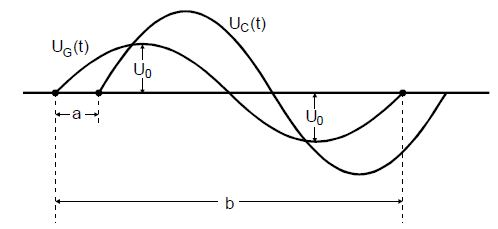
\includegraphics[height=5cm]{phase.JPG}
  \caption{Darstellung der Phasenverschiebung}
  \cite{skript2}.
  \label{fig:phase}
\end{figure}
Um die Phasenverschiebung zu bestimmen, genügt es den Wert $a$ (Abstand der Nulldurchgänge) zu messen, denn
$b$ (Periodenlänge) kann aus der Frequnz berechnet werden. Für die Frequenz werden die gleichen
Werte wie bei der Messung der Kondensatorspannung verwendet.





\label{sec:Durchführung}
